\documentclass[sigconf,nonacm]{acmart}
\settopmatter{printacmref=false,printfolios=true}
\setcopyright{none}
\renewcommand\footnotetextcopyrightpermission[1]{}
\usepackage{amsmath,tabularx,array,enumitem,balance,tikz,booktabs}
\usepackage{float}
\usetikzlibrary{arrows.meta,positioning,shapes.geometric}
\definecolor{CourseBlue}{HTML}{315EFB}
\definecolor{CourseTeal}{HTML}{14877D}
\definecolor{CourseInk}{HTML}{18324A}
\hypersetup{colorlinks=true,linkcolor=CourseBlue,citecolor=CourseTeal,urlcolor=CourseTeal}
\newcolumntype{Y}{>{\raggedright\arraybackslash}X}
\setlist{leftmargin=*,topsep=3pt,itemsep=2pt}

\newcommand{\CourseNumber}{COMSCI/ECON 206}
\newcommand{\CourseName}{Computational Microeconomics}
\newcommand{\CourseSession}{Autumn 2026 Session 1}
\newcommand{\Instructor}{Professor Luyao Zhang}
\newcommand{\TeamCode}{FP3}

\newcommand{\SymposiumSession}{September~28, 2:45--5:15 p.m., IB 2050}

\newcommand{\GitHubLink}{\url{https://github.com/dku-comsci-econ206-Autumn2026/ps2-fp3}}

\newcommand{\NotebookLink}{\url{https://colab.research.google.com/drive/11HK1McahmEDVwZfS208nEMeVkMAyVUil}}

\newcommand{\HuggingFaceLink}{\url{https://huggingface.co/spaces/dku-comsci-econ206-2026/strategic-disclosure-game}}

\newcommand{\PosterLink}{submitted separately as PPTX and PDF; no public URL}

\newcommand{\coursemeta}{\noindent\textbf{Submission to:} \CourseNumber{} --- \CourseName.\\
\textbf{Course session:} \CourseSession. \textbf{Team:} \TeamCode. \textbf{Symposium:} \SymposiumSession.\\
\textbf{Course instructor:} \Instructor. \textbf{Assignment:} PS2 collaborative research proposal.\\
\textbf{Artifacts:} GitHub: \GitHubLink. Colab: \NotebookLink. Hugging Face: \HuggingFaceLink. Poster: \PosterLink.\par\smallskip}

\title{Learning from Its Own Footprint: Strategic Disclosure, Capital Feedback, and the Design of AI Valuation Rules in IPO Allocation}

\author{Feiyu Li}
\affiliation{\institution{Duke Kunshan University}\city{Kunshan}\country{China}}
\email{feiyu.li@dukekunshan.edu.cn}

\author{Xuantong Fu}
\affiliation{\institution{Duke Kunshan University}\city{Kunshan}\country{China}}
\email{xuantong.fu@dukekunshan.edu.cn}

\renewcommand{\shortauthors}{Team \TeamCode}

\newif\ifTeachingAnnotations
\TeachingAnnotationsfalse

\begin{document}

\begin{teaserfigure}
\captionsetup{skip=8pt}
\centering
% PS2 teaser -- the feedback loop that defines this paper.
% Coordinate system is in points; \resizebox scales it to \textwidth.
\resizebox{\textwidth}{!}{%
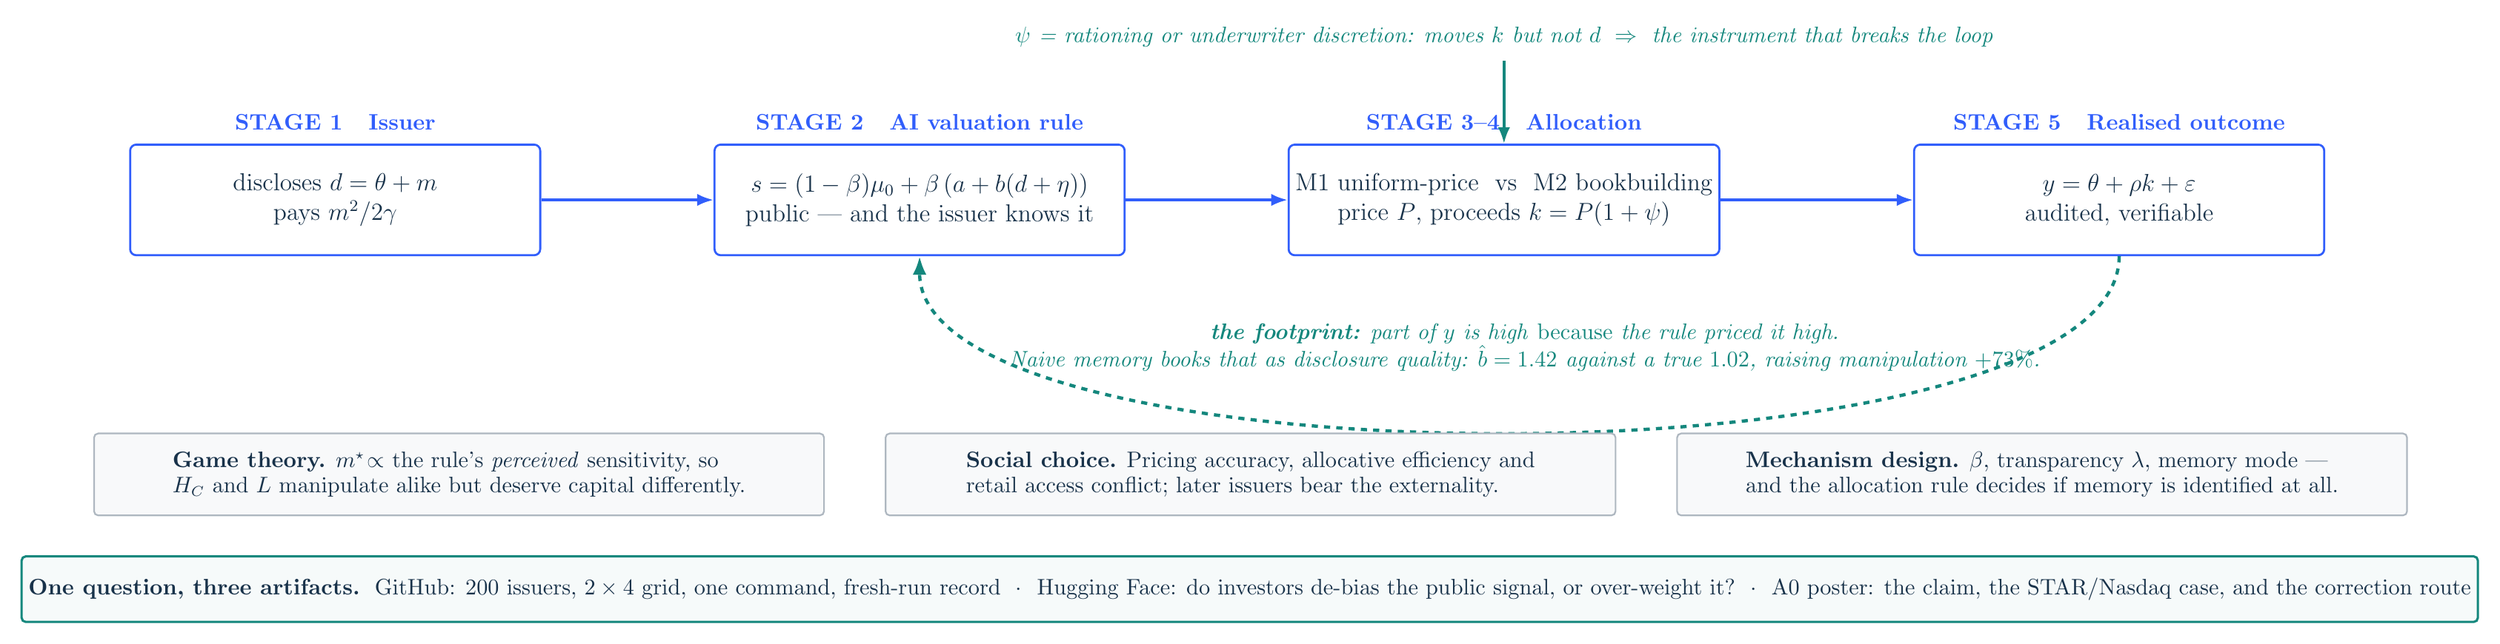
\begin{tikzpicture}[x=1pt,y=1pt,font=\sffamily,>=Latex]
\tikzset{
  stage/.style={draw=CourseBlue,line width=1.0pt,rounded corners=3pt,
                minimum width=200pt,minimum height=54pt,align=center,
                text=CourseInk,fill=white,font=\fontsize{12}{14.5}\selectfont},
  stagelab/.style={font=\bfseries\fontsize{11}{13}\selectfont,text=CourseBlue,align=center},
  flow/.style={CourseBlue,line width=1.3pt,-{Latex[length=8pt]}},
  loop/.style={CourseTeal,line width=1.6pt,-{Latex[length=9pt]},dashed},
  instr/.style={CourseTeal,line width=1.3pt,-{Latex[length=8pt]}},
  note/.style={font=\itshape\fontsize{11}{13.5}\selectfont,text=CourseTeal,align=center},
  lens/.style={draw=CourseInk!35,line width=0.8pt,rounded corners=2pt,
               minimum width=356pt,minimum height=40pt,align=left,
               text=CourseInk,fill=CourseInk!3,font=\fontsize{10.5}{12.5}\selectfont},
  synth/.style={draw=CourseTeal,line width=1.1pt,rounded corners=2pt,
                minimum width=1128pt,minimum height=32pt,align=center,
                text=CourseInk,fill=CourseTeal!4,font=\fontsize{11}{13}\selectfont}
}

% ---------- stage labels -------------------------------------------------
\node[stagelab] at (130,272) {STAGE 1 \ \ Issuer};
\node[stagelab] at (415,272) {STAGE 2 \ \ AI valuation rule};
\node[stagelab] at (700,272) {STAGE 3--4 \ \ Allocation};
\node[stagelab] at (1000,272) {STAGE 5 \ \ Realised outcome};

% ---------- the four stages ---------------------------------------------
\node[stage] (issuer)  at (130,234) {discloses $d=\theta+m$\\pays $m^{2}/2\gamma$};
\node[stage] (rule)    at (415,234) {$s=(1-\beta)\mu_{0}+\beta\,(a+b(d+\eta))$\\public --- and the issuer knows it};
\node[stage] (auction) at (700,234) {M1 uniform-price \ vs \ M2 bookbuilding\\price $P$, proceeds $k=P(1+\psi)$};
\node[stage] (outcome) at (1000,234) {$y=\theta+\rho k+\varepsilon$\\audited, verifiable};

\draw[flow] (issuer)--(rule);
\draw[flow] (rule)--(auction);
\draw[flow] (auction)--(outcome);

% ---------- the loop: the outcome feeds the rule's own memory ------------
\draw[loop] (outcome.south) to[out=-90,in=-90,looseness=0.5] (rule.south);
\node[note] at (710,162)
  {\textbf{the footprint:} part of $y$ is high \emph{because} the rule priced it high.\\
   Naive memory books that as disclosure quality: $\hat b=1.42$ against a true $1.02$,
   raising manipulation $+73\%$.};

% ---------- the instrument ----------------------------------------------
\draw[instr] (700,302)--(auction.north);
\node[note,anchor=south] at (700,305)
  {$\psi$ = rationing or underwriter discretion: moves $k$ but not $d$ $\;\Rightarrow\;$
   the instrument that breaks the loop};

% ---------- three lenses -------------------------------------------------
\node[lens,anchor=west] (l1) at (12,100)
  {\textbf{Game theory.} $m^{\star}\!\propto$ the rule's \emph{perceived} sensitivity, so\\
   $H_{C}$ and $L$ manipulate alike but deserve capital differently.};
\node[lens,anchor=west] (l2) at (398,100)
  {\textbf{Social choice.} Pricing accuracy, allocative efficiency and\\
   retail access conflict; later issuers bear the externality.};
\node[lens,anchor=west] (l3) at (784,100)
  {\textbf{Mechanism design.} $\beta$, transparency $\lambda$, memory mode ---\\
   and the allocation rule decides if memory is identified at all.};

% ---------- artifact bar -------------------------------------------------
\node[synth] at (576,44)
  {\textbf{One question, three artifacts.}\ \ GitHub: 200 issuers, $2\times4$ grid, one command, fresh-run record\ \
   $\cdot$\ \ Hugging Face: do investors de-bias the public signal, or over-weight it?\ \
   $\cdot$\ \ A0 poster: the claim, the STAR/Nasdaq case, and the correction route};
\end{tikzpicture}}


\caption{The loop this paper studies. The issuer manages the disclosure the rule reads; the rule's output affects capital allocation; capital changes realised outcomes; and those outcomes can enter the rule's later history. The current simulation reports a higher learned sensitivity and more manipulation under naive memory. Breaking the feedback requires variation in proceeds that is plausibly orthogonal to disclosure. Each lens below changes the analysis rather than merely labelling it.}

\Description{A four-stage flow across the top: the issuer discloses d equals theta plus m at quadratic cost; the AI valuation rule publishes a public signal s; a uniform-price auction or bookbuilding sets the price and proceeds; and the realised outcome y equals theta plus rho times capital plus noise. A dashed arrow runs from the realised outcome back into the AI rule, marking the feedback loop in which the rule trains on outcomes its own pricing produced. A separate arrow marks the allocation shock psi entering the auction stage as the instrument that identifies the capital effect. Beneath sit three lens panels for game theory, social choice, and mechanism design, and a bar naming the three linked artifacts.}

\label{fig:teaser}
\end{teaserfigure}

\maketitle
\raggedbottom
\coursemeta

\section{Research question and verified gap}
AI-assisted equity valuation creates a strategic environment: an issuer chooses what to disclose, an evaluator converts that disclosure into a public valuation signal, and investors use the signal when allocating scarce capital. The issuer knows the evaluator's rule, so disclosure is potentially strategic. The deeper problem begins when the evaluator learns from later firm outcomes. If its own valuation affects how much capital a firm receives, and capital affects later performance, then part of the evaluator's training data is generated by the evaluator itself.

\textbf{Shared question.} \emph{When firms know how an AI evaluator scores their disclosures, can a history-aware evaluator and an auction-based capital-allocation mechanism reduce strategic disclosure while preserving informative pricing?}

We answer this through three connected questions. \textbf{Q1--strategic behavior:} how does a firm respond when it knows the evaluator and the evaluator's output affects capital? \textbf{Q2--mechanism and computation:} can evaluator learning separate genuine firm quality from performance caused by its own allocation? \textbf{Q3--behavior:} do investors remove predictable disclosure inflation from the AI signal, as the equilibrium benchmark assumes?

\textbf{Verified gap.} Costly-disclosure models study strategic reporting under a fixed evaluation rule~\cite{lacker1989,crocker2007}. IPO research studies uniform-price auctions and bookbuilding as information and allocation mechanisms~\cite{benveniste1989,sherman2005,degeorge2007}. Performativity work studies how deployed predictors change the environment they predict~\cite{perdomo2020}. These literatures do not jointly model a predictor that both affects capital allocation and later learns from outcomes partly caused by that allocation. Our bounded gap is therefore the feedback loop, not the generic claim that ``AI matters in finance.''

\section{Strategic model and solution concept}
There are sequential issuers $t=1,\ldots,N$, investors, and a mechanism designer. Issuer $t$ privately knows fundamental quality $\theta_t$, private value of capital $v_t$, and social marginal product of capital $\rho_t$. It chooses disclosure
\begin{equation}
d_t=\theta_t+m_t, \qquad c(m_t)=m_t^2/(2\gamma).
\end{equation}
The evaluator publishes
\begin{equation}
s_t=(1-\beta)\mu_0+\beta\,[a+b(d_t+\eta_t)],
\end{equation}
where $b$ is the learned disclosure sensitivity. Investors observe $s_t$ and private signals $x_{it}=\theta_t+\xi_{it}$, then bid. The allocation rule determines price $P_t$ and proceeds $k_t$. Finally,
\begin{equation}
y_t=\theta_t+\rho_t k_t+\varepsilon_t
\end{equation}
becomes part of the history used for later calibration.

The information structure is incomplete because $\theta_t,v_t,\rho_t$ are private types, and imperfect because manipulation $m_t$ is not directly observed. The game is sequential, so we use \textbf{Perfect Bayesian Equilibrium}~\cite{harsanyi1968}. Under the quadratic cost and single-crossing condition, the firm's best response is increasing in the evaluator's perceived sensitivity:
\begin{equation}
m_t^\star=\gamma v_t n\lambda_P[\lambda\beta b+(1-\lambda)\kappa_0].
\end{equation}
Thus revealing the evaluation rule changes behavior. The benchmark prediction is not that firms literally fool a fully rational evaluator: investors can anticipate average inflation. The economic cost can instead appear as resources spent to optimize for the machine.

\textbf{Challenge test.} If a history-aware evaluator learns a larger $b$ from outcomes it partly caused, then the best response above increases even when fundamental quality has not changed. This creates a falsifiable prediction: naive history should increase manipulation relative to a no-memory baseline.

\section{Social choice and design objective}
The social planner does not simply maximize AI prediction accuracy. The relevant stakeholders are issuers, institutional investors, retail investors, exchanges/regulators, and later issuers who inherit the evaluator's calibration. We therefore track three competing objectives:
\begin{enumerate}
\item \textbf{Informative pricing:} minimize error between market price and latent fundamental value.
\item \textbf{Allocative efficiency:} direct scarce capital toward firms with high social marginal product $\rho$.
\item \textbf{Manipulation and access:} reduce disclosure-management waste while preserving meaningful retail participation.
\end{enumerate}
These objectives can conflict. A mechanism that produces strong institutional information may reduce retail access; a transparent evaluator may improve accountability while also making the target easier to manipulate. The project therefore reports a trade-off rather than a single ``best'' rule.

The feedback loop also creates an intertemporal externality: one issuer's strategic disclosure can change the evaluator's future calibration for later issuers. A socially acceptable evaluator should therefore distinguish genuine information from performance induced by its own previous allocations.

\section{Mechanism design and auction comparison}
The scarce resource is 100 shares in an IPO-style offering. We compare two consequential allocation rules. \textbf{M1: uniform-price auction} sorts price--quantity bids and allocates until shares are exhausted; winners pay the lowest accepted price. \textbf{M2: bookbuilding} uses investor indications and underwriter discretion, with the current model assigning 85\% of allocation to institutions and applying an 8\% pricing discount. These are deliberately different mechanisms, not two labels for the same rule.

The key innovation is that the auction also creates variation in proceeds. Write the observed outcome as $y=\theta+\rho k+\varepsilon$. A naive learner that regresses outcome on disclosure obtains
\begin{equation}
\hat b_{naive}=b_{true}+\rho\frac{\operatorname{Cov}(k,d)}{\operatorname{Var}(d)}+R,
\end{equation}
where the middle term is the evaluator's own capital footprint and $R$ captures remaining heterogeneity. We therefore compare three evaluator modes: \textbf{no memory}, \textbf{naive history}, and \textbf{capital-purged history}. The last uses allocation variation as an instrument for $k$ and is gated by a first-stage strength check.

This makes mechanism design consequential. The question is not merely which auction raises more revenue. It is whether the allocation rule supplies enough credible variation to identify the feedback that the evaluator must remove before learning from outcomes. The analogy boundary is explicit: real bookbuilding also includes certification and relationship effects that our controlled model does not represent.

\section{Computational and behavioral test}
The computational design uses 200 synthetic issuers, 10 cohorts, seeds 42--46, 100 shares per offering, 15 institutional and 35 retail investors, and the same disclosure, signal, memory, and auction rules described above. The primary outcomes are mean manipulation $\bar m$, price RMSE, capital-allocation efficiency, feedback bias $\hat b-b_{true}$, manipulation cost, retail allocation share, and the first-stage $F$ statistic.

The current simulation reports, for example, $\hat b=1.42$ versus $b_{true}=1.02$ under naive memory and an increase in mean manipulation from 0.233 to 0.402. The current bookbuilding condition produces substantially stronger allocation-shock variation than the uniform-price condition. These are model outputs, not evidence about real issuers; all reported numbers must be regenerated from the final code and seed record before submission.

The behavioral artifact tests the equilibrium assumption that investors remove predictable disclosure inflation from the public AI signal. A competing explanation is anchoring or algorithm appreciation~\cite{logg2019}. Players therefore face the same strategic setting as the model and their implied weight on the public signal is compared with the Bayesian benchmark. Classroom/Hugging Face evidence is exploratory: it can challenge or qualify the behavioral assumption but cannot establish population-level investor behavior.

\textbf{Integrated contribution.} Game theory predicts strategic disclosure; social choice defines the collective objectives and trade-offs; mechanism design changes the allocation rule and the information available for evaluator learning; computation tests the feedback mechanism; and behavioral play challenges the rational-investor benchmark. The practical implication is testable: any AI system that both evaluates and influences capital should expose enough of its calibration path and allocation footprint for an external auditor to distinguish genuine performance from performance it helped create.


\clearpage

\section*{Author Notes}
\subsection*{Acknowledgements}
We thank \textbf{Prof. Luyao Zhang} for incubating our research from its strategic-disclosure starting point through the interdisciplinary development of PS2, for her formal PS1 feedback, and for her immediate collaborative-learning feedback on evaluator commitment, revisability, and the need to make the evaluator's rule and correction path explicit. We thank \textbf{Prof. Ken Rogerson} for his discussions and course guidance. We thank \textbf{Han Zhang}, Liberata founder and Duke University Ph.D. Candidate, for his feedback on the accountability problem: when an AI evaluator makes consequential errors, the system needs an explicit correction or punishment route rather than treating the evaluator as automatically self-correcting. We thank our peer reviewers, \textbf{Aaron Wang} and \textbf{Zhenning Wang}, for their evidence-based comments on behavioral sample size, synthetic-data limitations, and identification under endogenous allocation shocks. We thank the \textbf{COMSCI/ECON 206 classroom community} for collaborative learning, questions, and discussion. We build on published work by Lacker and Weinberg~\cite{lacker1989}, Crocker and Slemrod~\cite{crocker2007}, Cao, Jiang, Yang and Zhang~\cite{cao2023machine}, Benveniste and Spindt~\cite{benveniste1989}, Sherman~\cite{sherman2005}, Degeorge, Derrien and Womack~\cite{degeorge2007}, Perdomo et al.~\cite{perdomo2020}, Staiger and Stock~\cite{staiger1997}, and Logg, Minson and Moore~\cite{logg2019}; none of these authors was involved in this work. Software used includes Python 3.11, NumPy, pandas, Matplotlib, and Gradio. The ACM \texttt{acmart} class and course template are used as provided. Generative AI assistance is disclosed in Appendix~A.1. Feedback or a program role does not imply coauthorship. The authors remain responsible for the proposal and remaining errors.

\subsection*{Team and individual contributions}
\textbf{Joint contribution.} We formulate a single feedback problem linking strategic disclosure, AI valuation, capital allocation, and subsequent AI learning. The common contribution is the design of a setting in which an issuer knows the evaluator, the evaluator's signal affects the auction outcome, capital changes the issuer's later performance, and that performance becomes part of the evaluator's history. This makes the evaluator's own allocation footprint an object of analysis rather than treating valuation and allocation as separate modules. The team jointly specifies the three connected questions, the strategic environment, the social-planner objectives, the auction comparison, the accountability extension, and the computational/behavioral tests. The resulting argument is: game theory predicts disclosure and bidding responses; social choice defines the trade-off among informative pricing, allocative efficiency, access, and accountability; and mechanism design changes the allocation rule and therefore the information available for safe history-based calibration.

\textbf{Feiyu Li (author 1).} \emph{Personal intellectual decision:} reframing the project around the joint design problem of an AI evaluator and a capital-allocation mechanism, with particular attention to the distinction between genuine firm quality and performance induced by capital allocated through the evaluator. \emph{Inspectable output:} the strategic-disclosure formulation, issuer-type specification, auction interface, behavioral-game design, and Sections~1, 2, 4, and 5. \emph{Verification and result:} independently re-ran the stated mechanism-by-memory comparison on seeds 42--46 and checked the sign and magnitude of the reported change in manipulation under naive historical learning. Feiyu also checked the investor-side interpretation of the public signal against the Bayesian benchmark. \emph{Connection:} this work connects the firm's disclosure incentive to the auction and to the behavioral test rather than treating them as separate examples. \emph{Next responsibility:} verify the final computational implementation against the behavioral interface and document any revision to the evaluator, auction, or accountability assumptions.

\textbf{Xuantong Fu (author 2).} \emph{Personal intellectual decision:} identifying the evaluator's own capital allocation as the source of a feedback/omitted-variable problem and making the allocation mechanism consequential for whether that footprint can be separated from true firm quality. \emph{Inspectable output:} the memory/update estimators, allocation-shock identification argument, auction comparison, bias decomposition, and supporting technical derivations in Section~3 and Appendix~A. \emph{Verification and result:} checked the analytic footprint component against the simulated allocation-induced outcome and verified the first-stage diagnostic used to decide whether capital-purged estimation is informative. \emph{Connection:} this identification work turns the auction comparison into part of the evaluator-design problem: a mechanism is useful not only because it allocates shares, but also because its variation determines what the evaluator can safely learn from. \emph{Next responsibility:} complete robustness checks for allocation-shock assumptions and test the proposed audit-triggered correction rule.

\textbf{Documented cross-check.} Each author independently verifies a consequential component of the other's work. Feiyu checks the computational outputs and behavioral-interface mapping from a clean checkout; Xuantong recomputes the core manipulation, price-informativeness, and allocation-efficiency measures and checks that their interpretation matches the stated social objective. Both authors review the consistency of the theory, simulation, behavioral artifact, and paper before submission.
\clearpage
\section{Technical details and reproducibility}
\textbf{Separating-equilibrium benchmark.} With $c(m)=m^2/2\gamma$ and a linear price response, the cost of increasing the report is convex. The single-crossing condition supports a separating benchmark in which the optimal manipulation is increasing in the evaluator's perceived sensitivity to disclosure. The exact expression used in the simulation is
\begin{equation}
m^\star=\gamma\, v\, n\,\lambda_P\,\big[\lambda\beta b+(1-\lambda)\kappa_0\big].
\label{eq:br-app}
\end{equation}
This is the strategic link between evaluator design and disclosure cost; it is not interpreted as an empirical estimate of any real issuer.

\textbf{Feedback decomposition.} The simulated learning problem can be written as
\begin{equation}
\hat b-b_{\text{true}}=\rho\,\frac{\operatorname{Cov}(k,d)}{\operatorname{Var}(d)}+R,
\label{eq:bias-app}
\end{equation}
where the first term is the capital footprint targeted by the allocation-shock correction and $R$ collects remaining heterogeneity. In the current model the footprint is generated by the mechanism; therefore the correction is only as credible as the instrument assumptions. The unresolved residual is explicitly treated as a limitation and planned robustness target rather than as a solved empirical problem.

\textbf{Language-independent pseudocode.}
\begin{verbatim}
for seed in {42,...,46}:
    initialize issuer types and private signals
    for issuer in sequential_IPOs:
        choose disclosure d from strategic best response
        compute public AI signal s from memory mode
        collect investor bids from private + public information
        P, allocation, psi <- run_auction(bids, mechanism)
        k <- proceeds_per_share(P, psi)
        y <- theta + rho*k + noise
        update evaluator memory using mode
aggregate RMSE, manipulation, allocation efficiency,
price error, welfare, retail access, and bias diagnostics
\end{verbatim}

\textbf{Inputs and parameters.} The computational design uses $N=200$ issuers (10 cohorts $\times$ 20), 100 shares per offering, seeds 42--46, a two-cohort burn-in, $\sigma_\theta=1.0$, $\gamma=0.006$, $\sigma_\eta=0.5$, $\mu_0=8.5$, $\beta=0.60$, $\lambda=1.0$, and $\sigma_\varepsilon=0.8$. The investor pool contains 15 institutions ($\sigma_\xi=1.0$) and 35 retail investors ($\sigma_\xi=2.5$). The calibrated issuer parameters are $v\sim N(2.2,0.4^2)$ and $\rho\sim N(0.50,0.12^2)$, truncated at positive values; $b_{\text{true}}=1.02$, $\lambda_P=1.0$, and $\kappa_0=0$. The allocation-shock standard deviation is 0.08 for uniform-price allocation and 0.20 for bookbuilding; bookbuilding assigns 85\% of shares to institutions and applies an 8\% pricing discount. These values are copied from the computational configuration used for the fresh Colab run.

\textbf{Metrics.} Primary outcomes are (i) manipulation, $\bar m$ and manipulation cost; (ii) price informativeness, measured by RMSE between the transaction price and the latent fundamental value; (iii) capital-allocation efficiency, measured by the relationship between capital and $\rho$; and (iv) evaluator feedback bias, $\hat b-b_{\text{true}}$, with its footprint decomposition. Secondary outcomes include retail allocation share, realised investor return, and the first-stage $F$ statistic for the allocation-shock correction.

\textbf{Known limitations.} (1) $\rho$ is exogenous; the model does not solve a dynamic general-equilibrium problem. (2) Memory is cross-firm rather than cross-period, so the model is an abstraction of repeated calibration rather than a literal representation of seasoned issuance. (3) The AI is represented as a rule rather than as a strategic vendor with its own payoff. (4) Only one evaluator is modelled; competing valuation systems are left for future work. (5) The heterogeneity residual $R$ in Eq.~\eqref{eq:bias-app} is unresolved. (6) All data are synthetic; no claim is made about any real issuer. (7) Behavioral evidence is exploratory and cannot establish population-level investor behavior.

\textbf{Actual versus planned evidence.} The numerical values labelled ``actual'' in this version are outputs of the fresh Colab run using the five canonical Python files, seeds 42--46, and the stated burn-in rule. They are synthetic simulation results, not empirical evidence about real issuers. Robustness checks beyond the reported treatment grid remain planned. The classroom/Hugging Face behavioral test and post-symposium review response are kept separate from these computational results and are not represented as completed here.

\textbf{Fresh-run record.} Review-ready artifacts are currently linked at the GitHub repository \url{https://github.com/dku-comsci-econ206-Autumn2026/ps2-fp3}, the Colab notebook \url{https://colab.research.google.com/drive/1o-t9W3shjHubzSBcB8QK6KYFumrJmEbh}, and the Hugging Face Space \url{https://huggingface.co/spaces/dku-comsci-econ206-2026/strategic-disclosure-game}. The A0 poster is submitted separately as PPTX and PDF. The exact Git commit/release, Space revision, UTC timestamp, Python/package versions, seed list, and regeneration command will be frozen in the final clean-run record.

\subsection{AI-use disclosure}
The team used OpenAI ChatGPT (GPT-5.6 Luna) during September~2026 for research-question refinement, mathematical-model clarification, LaTeX drafting and debugging, Python implementation and debugging, Hugging Face interface development, Colab/notebook organization, and poster editing. The authors independently chose the research question, strategic environment, evaluator modes, auction comparison, objectives, and core model before accepting generated drafts or code. Suggestions were treated as drafts: the authors rejected or revised suggestions that did not match the project design, and they checked equations, file consistency, simulation logic, artifact behavior, links, and final claims. Generative AI was not treated as a source of empirical evidence. The human authors remain responsible for all claims, citations, computations, and submitted artifacts.

\clearpage
\section{Cumulative Intellectual Development}
\textbf{Prior methodological starting point.} The project began from the course's strategic-disclosure setting. The PS2 revision adds a consequential allocation mechanism and a history-learning loop rather than treating the evaluator as a static scoring rule.

\textbf{Revision path.} The key change was to make the evaluator's output affect capital allocation and then make realised performance feed back into the evaluator. This created a testable distinction between genuine information in disclosure and performance induced by the evaluator's own decisions. The auction comparison was then made part of the identification problem rather than a decorative application.

\textbf{Intellectual consequence.} Asking whether the evaluator learns from outcomes it caused changed the central question from ``can firms manipulate the AI?'' to ``how should an evaluator learn when its own pricing changes the data-generating process?'' This change affects the strategic model, social objective, mechanism comparison, computational metrics, and behavioral interface.

\section{Open-source and three-lens inspiration}
\textbf{Strategic/game-theoretic foundation.} Harsanyi~\cite{harsanyi1968} supplies the incomplete-information equilibrium logic, while costly-state-falsification models~\cite{lacker1989,crocker2007} motivate strategic disclosure. These foundations lead us to model private issuer types, disclosure costs, sequential moves, and beliefs explicitly.

\textbf{Social-choice foundation.} The social planner does not have a single objective. Informative prices, efficient allocation of scarce capital, disclosure costs, and access for retail investors can conflict. The project therefore treats welfare as a multi-objective design problem and reports the trade-off rather than collapsing it into one accuracy statistic.

\textbf{Mechanism-design foundation.} Myerson~\cite{myerson1981} and the auction literature motivate comparing allocation/payment rules. The consequential design decision here is whether the mechanism creates usable variation in proceeds without changing the issuer's disclosure decision directly. This is why the auction comparison enters the evaluator-learning problem.

\textbf{Computational and behavioral integration.} GitHub makes the simulation reconstructable; Hugging Face makes the behavioral assumption about investor reliance observable; the A0 poster must integrate the same question, evidence, limitations, and real-world case. Behavioral play is treated as a challenge test of the equilibrium benchmark, not as population validation.

\section{Formal response to feedback and revision map}
This appendix is the team's formal response map for PS2. Each entry records the source, the point raised, our decision, the concrete change, the evidence location, and the remaining question. Reviewer sheets are not reproduced here.

\begin{tabularx}{\columnwidth}{@{}p{1.35cm}Y@{}}\toprule
\textbf{Source} & \textbf{Response map} \\\midrule
Prof. Luyao Zhang --- formal PS1 feedback & \textbf{Point:} the original question should connect manipulable AI signals to real value, and the next step should ask when evaluator memory can substitute for commitment; compare fixed and revisable evaluator rules. \textbf{Decision: Adapt.} \textbf{Change:} Sections~2--4 now distinguish a fixed no-memory rule from revisable history-aware rules and add an explicit audit-triggered freeze/review correction path. \textbf{Evidence:} Sections~2--4 and the ``Cumulative Intellectual Development'' section. \textbf{Remaining question:} whether commitment or correction changes disclosure and pricing outcomes; planned as a future treatment.\\
Prof. Luyao Zhang --- immediate collaborative-learning feedback & \textbf{Point:} make the evaluator's rule, its revisability, and its consequences inspectable rather than treating ``AI learning'' as an automatic improvement. \textbf{Decision: Accept.} \textbf{Change:} the paper now states the fixed-versus-revisable distinction, labels the correction mechanism as proposed rather than tested, and separates current simulation evidence from planned accountability tests. \textbf{Evidence:} Sections~2 and~5; Appendix ``Technical details and reproducibility.'' \textbf{Remaining question:} what error threshold and review rule would be credible without creating new manipulation incentives? Planned.\\
Aaron Wang --- peer review & \textbf{Point:} the behavioral section did not report a completed sample size or actual treatment results, and the allocation-shock exogeneity should be checked. \textbf{Decision: Revise + Investigate.} \textbf{Change:} we removed any implication of completed population-level behavioral evidence, explicitly label the Hugging Face/classroom test exploratory, require completed $n$ and matched treatment outputs before stronger claims, and retain the first-stage/exogeneity limitation. \textbf{Evidence:} Section~5; Appendix ``Known limitations'' and ``PS2 extension record.'' \textbf{Remaining question:} whether the allocation-shock correction remains valid when shocks are endogenous; planned preregistered/controlled robustness test.\\
Zhenning Wang --- peer review & \textbf{Point:} the game rules and mechanism comparison are clear, but the current evidence is synthetic and therefore may not generalize to real IPO markets; test heterogeneous issuers and real issuance settings. \textbf{Decision: Investigate.} \textbf{Change:} the manuscript now states explicitly that all reported numerical evidence is synthetic, limits the interpretation of the 70\%/history effects to the model, and adds real-IPO replication with heterogeneous issuers as a future verification target. \textbf{Evidence:} Section~5; Appendix ``Known limitations'' and ``Actual versus planned evidence.'' \textbf{Remaining question:} whether the same feedback footprint appears with real issuance data and heterogeneous issuers; planned.\\
Han Zhang --- Liberata founder and Duke Ph.D. candidate & \textbf{Point:} if an AI evaluator makes consequential errors, the design should say how the system is corrected or penalized rather than assuming it can learn safely from its own outcomes. \textbf{Decision: Adapt.} \textbf{Change:} we add an audit-triggered freeze: when error is large and the allocation-footprint diagnostic indicates self-induced feedback, the update is frozen and the last audited parameter is restored; repeated failures trigger human review. This is explicitly a proposed accountability mechanism, not a tested result. \textbf{Evidence:} Section~2 ``Commitment and correction extension''; Section~3 social-choice objective; Section~5 integrated contribution; Appendix ``PS2 extension record.'' \textbf{Remaining question:} how to set the error threshold and penalty without creating incentives to manipulate the audit itself; planned.\\
\bottomrule
\end{tabularx}

\smallskip\noindent\textbf{Response status.} The substantive comments above are incorporated as model/argument revisions or explicitly bounded future tests. No unobserved behavioral sample size, real-IPO result, or successful correction effect is claimed as current evidence. The exact computational outputs remain those regenerated from the canonical simulation settings and seeds 42--46.

\clearpage\onecolumn
\section{Structured abstract and cumulative proposal map}\label{app:abstract}
\par\medskip
\begin{table}[H]
\caption{Structured abstract, PS2.}
\label{tab:abstract-map}
\renewcommand{\arraystretch}{1.18}
\begin{tabularx}{\textwidth}{@{}p{0.25\textwidth}Y@{}}\toprule
\textbf{Proposal element} & \textbf{Current statement / change} \\\midrule
Background & Investors increasingly use automated valuation signals built from issuer disclosures. Strategic disclosure can distort what machine readers observe~\cite{cao2023machine}; costly-state-falsification models study such incentives under fixed rules~\cite{lacker1989,crocker2007}. The unresolved setting here is a rule that both evaluates and affects capital allocation, so its later training data can partly reflect its own decisions. \\
Motivation and application & IPO-style capital allocation is used as a controlled mechanism-design environment. Stakeholders include issuers, institutional investors, retail investors, exchanges, regulators, and later issuers who inherit the evaluator's calibration. \\
Three connected questions & \emph{Economics:} how does strategic disclosure respond to a known evaluator? \emph{Computation:} can evaluator learning separate true quality from allocation-induced performance? \emph{Behavior:} do investors remove predictable disclosure inflation from the public signal? \emph{Integrated:} how should evaluator design and allocation design be jointly chosen? \\
Method and model assumptions & Private issuer types $(\theta,v,\rho)$; sequential disclosure, valuation, bidding, allocation, and outcome; PBE~\cite{harsanyi1968}; no-memory, naive-history, and capital-purged memory modes; uniform-price auction versus bookbuilding; 200 synthetic issuers and seeds 42--46. \\
\textbf{Results or expected results} & \textbf{Fresh simulation output:} history-aware evaluation produces substantially more manipulation and pricing error than no memory. Under uniform-price allocation, mean manipulation is 0.408, 1.367, and 1.277 for no memory, naive history, and capital-purged history; under bookbuilding it is 0.408, 0.921, and 1.002. Price RMSE is 0.551, 30.328, and 26.478 under uniform-price allocation and 0.776, 12.302, and 14.321 under bookbuilding. Feedback bias is 0.461, 5.344, and 4.894 under uniform-price allocation and 0.403, 2.012, and 2.527 under bookbuilding. The current purging rule therefore does not reliably eliminate feedback bias. \textbf{Planned verification:} test robustness to alternative signal noise, allocation shocks, and heterogeneous capital productivity. \\
Intellectual merits & The contribution is the feedback loop: the evaluator's signal affects capital, capital affects outcomes, and outcomes enter future calibration. The auction is consequential because its allocation variation determines whether that feedback can be separated from genuine disclosure information. \\
Practical impacts & A possible design standard is to require an AI valuation rule that also allocates capital to disclose its calibration path and the evidence separating evaluator-induced outcomes from genuine quality. Benefits, risks, access constraints, and correction routes remain design hypotheses until validated on external data. \\
Feedback received and revision made & The PS1/Week~4 starting point treated buyer behavior too mechanically. The PS2 revision makes investor bidding strategic and makes the auction consequential for both allocation and evaluator learning. The symposium feedback is now incorporated in the formal response map above; future challenges are labelled as planned tests. \\
\bottomrule
\end{tabularx}
\end{table}

\clearpage\twocolumn
\section{PS2 extension record: auction, linked artifacts, poster, and symposium}
\subsection{Auction laboratory record}
\textbf{Rules, stated explicitly.} \emph{Uniform-price (M1).} Allocation: bids are sorted descending and accepted until the 100-share offering is exhausted. Payment: winners pay the lowest accepted price. Stopping: cumulative demand reaches the offering. \emph{Bookbuilding (M2).} Allocation: underwriter discretion with the current model assigning 85\% to institutions. Payment: the model uses an underwriter price with an 8\% discount to the precision-weighted institutional estimate. Stopping: close of the book. The analogy boundary is explicit: real IPO bookbuilding also involves certification, relationship, and allocation considerations not represented here.

\begin{tabularx}{\columnwidth}{@{}p{1.45cm}Y@{}}\toprule
\textbf{Treatment}&\textbf{Setting, prediction, current output, revision status}\\\midrule
M1, no memory&Baseline. Current output: mean manipulation 0.408, manipulation cost 14.305, price RMSE 0.551, capital--$\rho$ correlation 0.055, feedback bias 0.461, retail share 70.0\%, and mean first-stage $F=0.310$.\\
M1, naive history&Predicted: outcome-based learning can amplify strategic disclosure. Current output: mean manipulation 1.367, manipulation cost 243.230, price RMSE 30.328, feedback bias 5.344, retail share 70.0\%, and $F=0.140$.\\
M1, purged history&Predicted: removing the capital footprint may reduce bias if the allocation variation is strong enough. Current output: mean manipulation 1.277, price RMSE 26.478, feedback bias 4.894, and $F=0.136$. The purged rule reduces bias relative to naive history here, but the first stage is weak and the bias remains large.\\
M2, no memory&Baseline bookbuilding condition. Current output: mean manipulation 0.408, manipulation cost 14.305, price RMSE 0.776, capital--$\rho$ correlation 0.037, feedback bias 0.403, retail share 15.0\%, and $F=2.287$.\\
M2, naive history&Predicted: outcome-based learning can amplify strategic disclosure. Current output: mean manipulation 0.921, manipulation cost 91.928, price RMSE 12.302, feedback bias 2.012, retail share 15.0\%, and $F=0.866$.\\
M2, purged history&Predicted: stronger allocation variation may help separate capital effects. Current output: mean manipulation 1.002, manipulation cost 107.819, price RMSE 14.321, feedback bias 2.527, retail share 15.0\%, and $F=0.900$. In this run, purging does not reduce feedback bias relative to naive history, so the proposed correction remains unresolved.\\
Classroom/HF&Classroom/HF behavioral test: record investor reliance on the public AI signal, compare it with the Bayesian benchmark, and treat the result as exploratory rather than population validation.\\\bottomrule
\end{tabularx}

\smallskip\noindent\textbf{Behavioral observation to record.} The main test is whether players remove predictable disclosure inflation from the AI signal. Algorithm appreciation~\cite{logg2019} and simple anchoring make competing predictions about how the weight on the public signal changes when the evaluator's calibration status is disclosed. The result will be labelled exploratory.

\subsection{Linked-artifact parity}
\begin{tabularx}{\columnwidth}{@{}p{1.45cm}Y@{}}\toprule
\textbf{Artifact}&\textbf{Parity check}\\\midrule
GitHub&Must implement the same issuer types, disclosure best response, memory modes, auction rules, parameters, and seeds as the paper. A clean run must regenerate every reported numerical table.\\
Hugging Face&Must expose the same decision setting used in the behavioral section: strategic disclosure, AI valuation, investor action, and allocation. The interface must not imply population-level behavioral validity.\\
A0 poster&Must use the same research question, core model, auction comparison, verified numerical outputs, limitations, real-world case, and correction route as the paper.\\\bottomrule
\end{tabularx}

\subsection{Symposium and practical-impact record}
\textbf{Symposium.} Session C. The manuscript, poster, repository, and behavioral artifact use the same research question and core model; behavioral observations remain exploratory unless a completed sample and matched outputs are recorded.

\textbf{Real-world case record.} The application is AI-assisted IPO/equity valuation and allocation. Affected stakeholders include genuine capital-constrained issuers, weaker issuers, institutional investors, retail investors, exchanges, regulators, and later issuers affected by the evaluator's history. Potential benefit: an auditable criterion for deciding when a valuation rule can safely learn from outcomes. Risk: a naive self-calibrated rule may look strong on backtests precisely because its errors track its own past allocations. Missing evidence: real issuance data with defensible allocation shocks. Correction route: publish the evaluator's calibration path, memory-update log, and identification diagnostics so an outside auditor can challenge the feedback assumption.

\textbf{Final revision record.} The formal response map above records the consequential feedback received for this revision. Future work is limited to the explicitly labelled robustness, real-IPO, and accountability tests.


\clearpage
\section*{References}
\begin{thebibliography}{99}
\bibitem{nash1950} John F. Nash. 1950. Equilibrium Points in n-Person Games. \emph{Proceedings of the National Academy of Sciences} 36, 1 (1950), 48--49. doi:10.1073/pnas.36.1.48.
\bibitem{harsanyi1968} John C. Harsanyi. 1968. Games with Incomplete Information Played by Bayesian Players, II: Bayesian Equilibrium Points. \emph{Management Science} 14, 5 (1968), 320--334. doi:10.1287/mnsc.14.5.320.
\bibitem{vickrey1961} William Vickrey. 1961. Counterspeculation, Auctions, and Competitive Sealed Tenders. \emph{The Journal of Finance} 16, 1 (1961), 8--37. doi:10.1111/j.1540-6261.1961.tb02789.x.
\bibitem{myerson1981} Roger B. Myerson. 1981. Optimal Auction Design. \emph{Mathematics of Operations Research} 6, 1 (1981), 58--73. doi:10.1287/moor.6.1.58.
\bibitem{un_sdg} United Nations. n.d. Sustainable Development Goals. https://sdgs.un.org/goals. Accessed September 21, 2026.
\bibitem{cao2023machine} Sean Cao, Wei Jiang, Baozhong Yang, and Alan L. Zhang. 2023. How to Talk When a Machine Is Listening: Corporate Disclosure in the Age of AI. \emph{The Review of Financial Studies} 36, 9 (2023), 3603--3642. doi:10.1093/rfs/hhad021.
\bibitem{sec2024aiwashing} U.S. Securities and Exchange Commission. 2024. SEC Charges Two Investment Advisers with Making False and Misleading Statements About Their Use of Artificial Intelligence. Press Release 2024-36. https://www.sec.gov/news/press-release/2024-36.
\bibitem{lacker1989} Jeffrey M. Lacker and John A. Weinberg. 1989. Optimal Contracts under Costly State Falsification. \emph{Journal of Political Economy} 97, 6 (1989), 1345--1363. doi:10.1086/261657.
\bibitem{crocker2007} Keith J. Crocker and Joel Slemrod. 2007. The Economics of Earnings Manipulation and Managerial Compensation. \emph{The RAND Journal of Economics} 38, 3 (2007), 698--713. doi:10.1111/j.0741-6261.2007.00107.x.
\bibitem{benveniste1989} Lawrence M. Benveniste and Paul A. Spindt. 1989. How Investment Bankers Determine the Offer Price and Allocation of New Issues. \emph{Journal of Financial Economics} 24, 2 (1989), 343--361. doi:10.1016/0304-405X(89)90051-2.
\bibitem{sherman2005} Ann E. Sherman. 2005. Global Trends in IPO Methods: Book Building versus Auctions with Endogenous Entry. \emph{Journal of Financial Economics} 78, 3 (2005), 615--649. doi:10.1016/j.jfineco.2004.09.005.
\bibitem{degeorge2007} François Degeorge, François Derrien, and Kent L. Womack. 2007. Analyst Hype in IPOs: Explaining the Popularity of Bookbuilding. \emph{The Review of Financial Studies} 20, 4 (2007), 1021--1058. doi:10.1093/rfs/hhm010.
\bibitem{perdomo2020} Juan C. Perdomo, Tijana Zrnic, Celestine Mendler-Dünner, and Moritz Hardt. 2020. Performative Prediction. In \emph{Proceedings of the 37th International Conference on Machine Learning (ICML)}, 7599--7609.
\bibitem{staiger1997} Douglas Staiger and James H. Stock. 1997. Instrumental Variables Regression with Weak Instruments. \emph{Econometrica} 65, 3 (1997), 557--586. doi:10.2307/2171753.
\bibitem{logg2019} Jennifer M. Logg, Julia A. Minson, and Don A. Moore. 2019. Algorithm Appreciation: People Prefer Algorithmic to Human Judgment. \emph{Organizational Behavior and Human Decision Processes} 151 (2019), 90--103. doi:10.1016/j.obhdp.2018.12.005.
\end{thebibliography}


\end{document}
